%!TEX root = lections.tex
Рассмотрим
\begin{equation}
	\pdv{U}{t}+U\pdv{U}{x}+\beta \pdv[3]{U}{x}-\nu\pdv[2]{U}{x}=0.
	\label{eq:45}
\end{equation}

$\nu>0$ - диссипация. К чему приведет ее учет?

Если $\beta=0$, то уравнение называется уравнением Бюргерса. 

$\xi=x-Vt$ - называют стационарным решением, т.к. профиль не меняется. 
\begin{equation*}
	-V\dv{U}{\xi}+U\dv{U}{\xi}+\beta\dv[3]{U}{\xi}-\nu\dv[2]{U}{\xi}=0.
\end{equation*}

Проинтегрируем:
\begin{equation*}
	\beta\dv[2]{U}{\xi}-\nu \dv{U}{\xi}+\frac{U^2}{2}-VU=0.
\end{equation*}
($\cdot$ - дифференцирование по $\xi$)
\begin{equation}
	\begin{cases}
		\dot{U}=y \\
		\beta \dot{y} =\nu y-\frac{U^2}{2}+VU.		
	\end{cases}
	\label{eq:46}
\end{equation}

Система определена на фазовой плоскости. Состояния равновесия: $O_1(0,0)$, $O_2(2V,0)$. Линеаризуем в этих точках. $O_1$ - седло, а для $O_2$:
\begin{gather*}
	p^2-\frac{\nu}{\beta}p+\frac{V}{\beta}=0, \\ p_{1,2}=\frac{\nu}{2\beta}\pm \sqrt{\frac{\nu^2}{4\beta^2}-\frac{V}{\beta}}.
\end{gather*}

Если $\frac{\nu^2}{4\beta^2}-\frac{V}{\beta}<0$, то имеем неустойчивый фокус.
\begin{equation*}
	\frac{\nu^2}{4\beta}=V \rightarrow \beta=\frac{\nu^2}{4V}.
\end{equation*}
\begin{figure}[H]
	\centering
	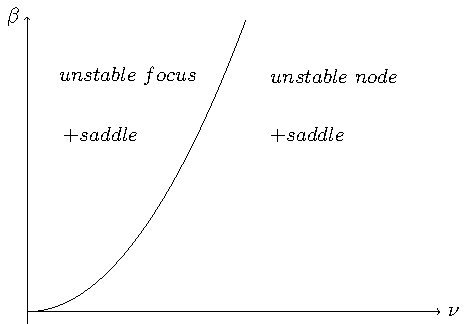
\includegraphics[width=0.4\linewidth]{fig/fig27.pdf}   
\end{figure}

Возьмем полную энергию при $\nu=0$:
\begin{equation*}
	V(U,y)=\beta\frac{y^2}{2}+\frac{U^3}{6}-V\frac{U^2}{2},
\end{equation*}

\begin{figure}[H]
	\centering
	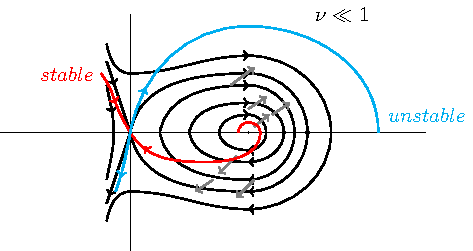
\includegraphics[width=0.4\linewidth]{fig/fig30.pdf}   
\end{figure}

\begin{equation*}
	\dot{V}=\beta y \dot{y}+\frac{U^2}{2}\dot{U}-VU\dot{U}=\nu y^2-\frac{U^2}{2}y+VUy-VUy+\frac{U^2}{2}y=\nu y^2\geqslant 0,
\end{equation*}
т.е. траектории системы пересекают линии уровня в сторону возрастания. Из существования этой функции следует, что система не имеет предельных циклов. 

Как ведут себя устойчивые сепаратрисы седла? Ограниченное решение существует, оно единственно и соответствует красной траектории. Зафиксируем $\beta$:
\begin{figure}[H]
	\centering
	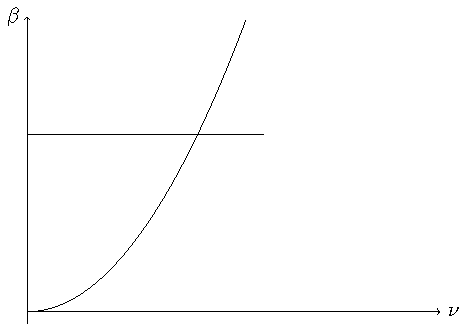
\includegraphics[width=0.4\linewidth]{fig/fig28.pdf}   
\end{figure}

Нарисуем профиль этой волны (для траектории, котора успеет сделать много витков, до того, как придет в состояние равновесия) ($\nu\ll1$):
\begin{figure}[H]
	\centering
	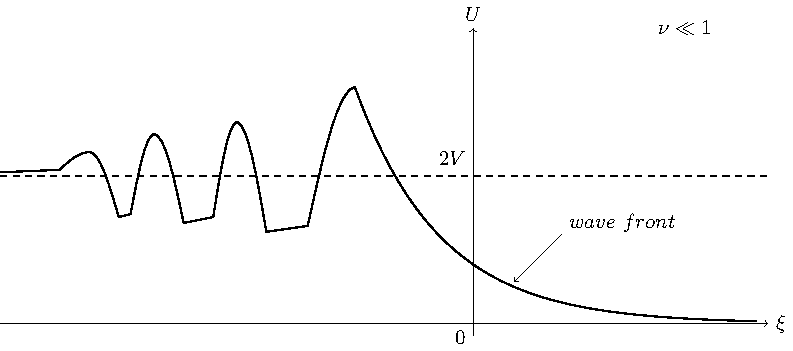
\includegraphics[width=0.6\linewidth]{fig/fig29.pdf}   
\end{figure}

Чем дальше от седла, тем ближе точки, выше и меньше полки. Это ударная волна.  Среда была в покое, прошел фронт и перебросил среду в новое состояние $2V$.

Для красной траектории:
\begin{figure}[H]
	\centering
	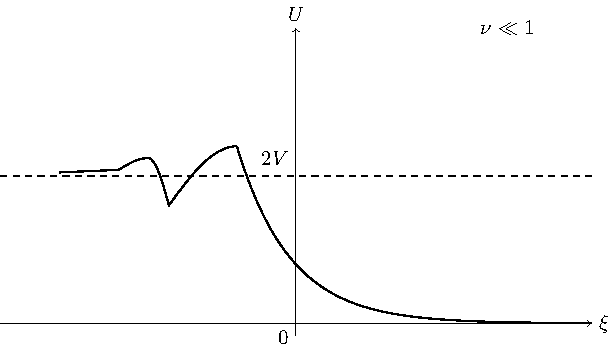
\includegraphics[width=0.6\linewidth]{fig/fig31.pdf}   
\end{figure}

Для траектории, идущей из неустойчивого состояния равновесия (фокуса или узла) в седло:
\begin{figure}[H]
	\centering
	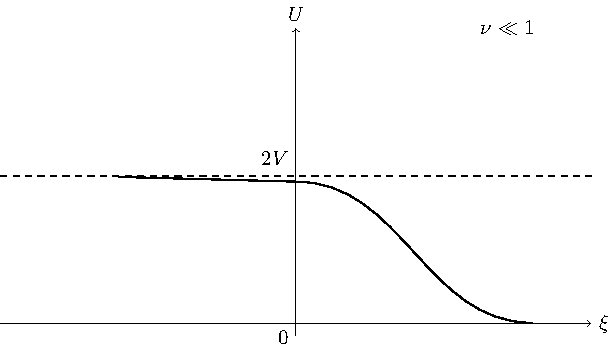
\includegraphics[width=0.6\linewidth]{fig/fig32.pdf}   
\end{figure}

Здесь не будет осцилляций. Во всех случаях есть передний фронт.
